\begin{equation}
	\centering
	P_L = \frac{ {\hat{V}_o}^{2} }{R_L} = \SI{1}{\watt} \implies \hat{V}_o = \sqrt{\SI{1}{\watt} \cdot \SI{8}{\ohm}} \implies \boxed{\hat{V}_o = \SI{4}{\volt}}
\end{equation}
La respuesta en frecuencia del circuito para una disipación de \SI{1}{\watt} ($\hat{V}_o = \SI{4}{\volt}$) en la carga se muestra en la Figura \ref{fig.rta_frec}.

%\begin{figure}[H]	
%	\centering
%	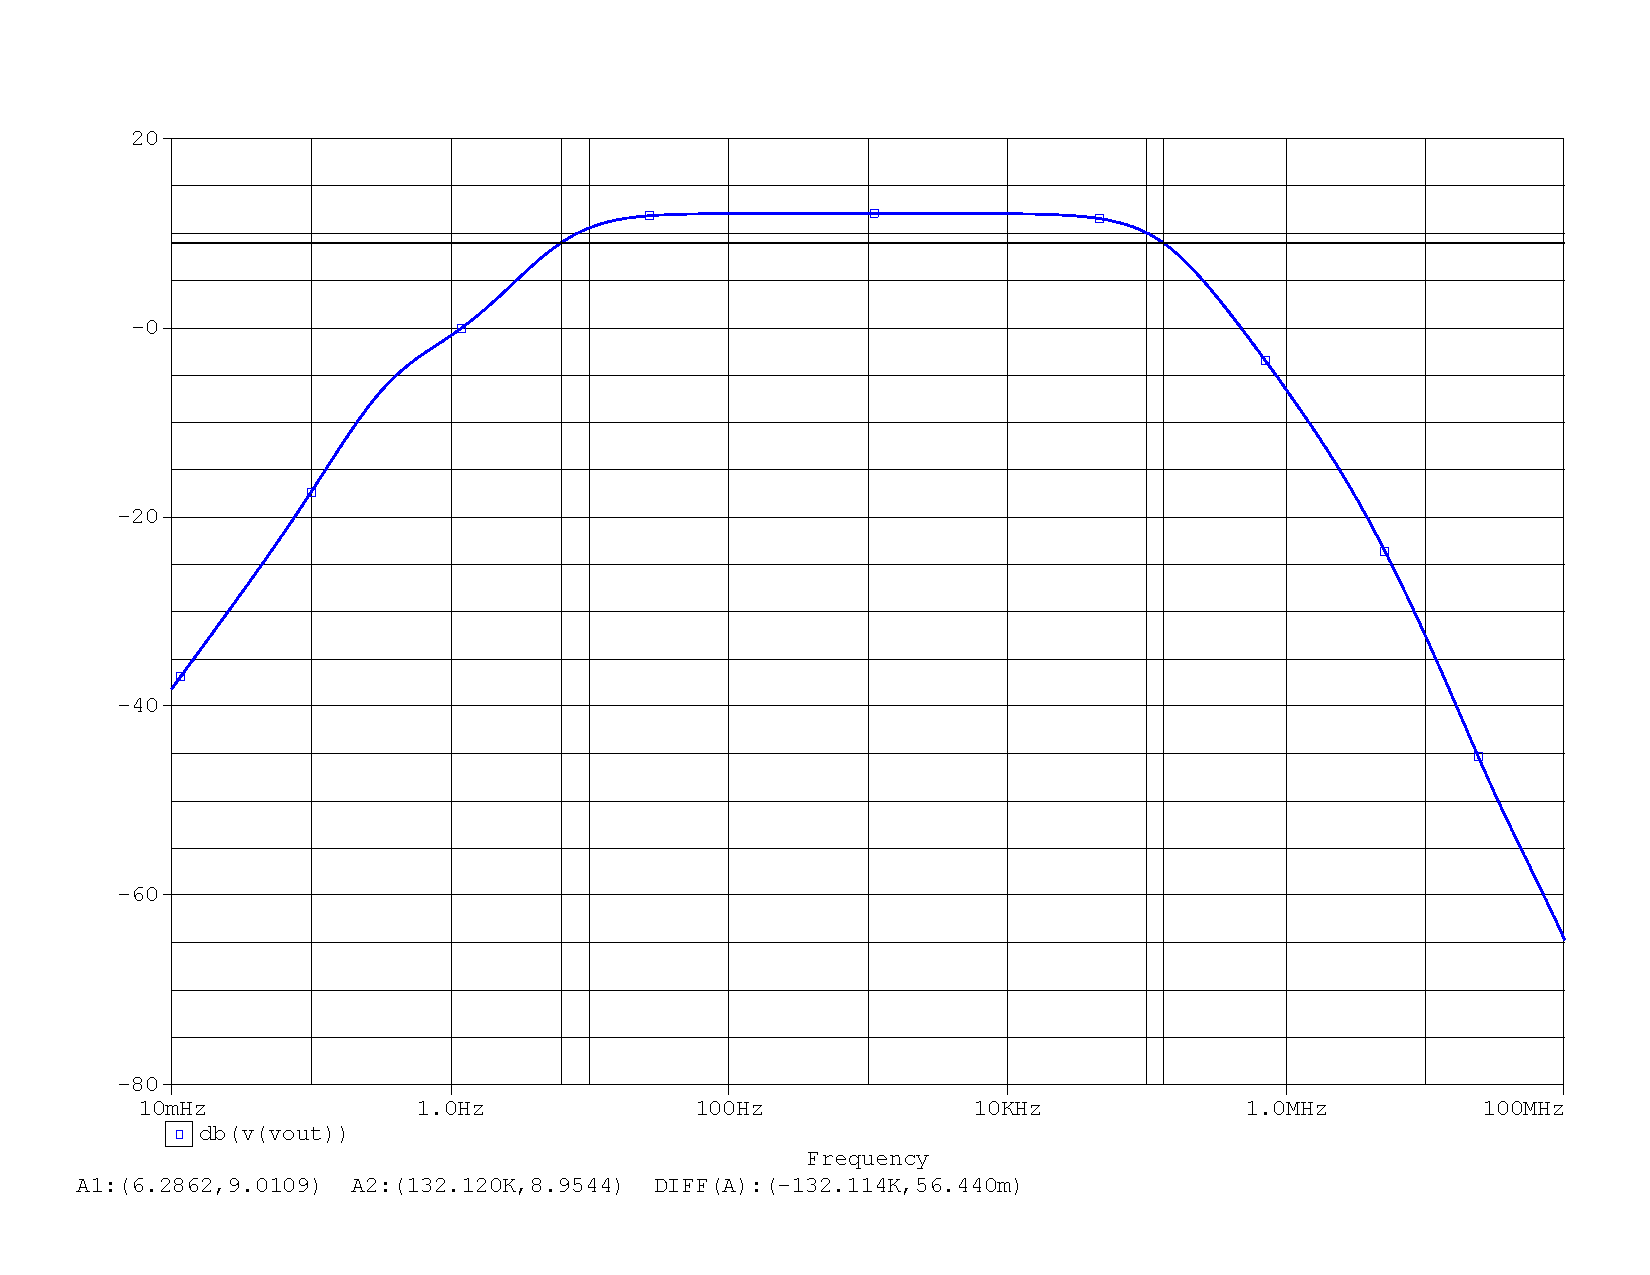
\includegraphics[scale=0.5]{sim_rta_frec_1W.pdf}
%	\caption{Respuesta en frecuencia del circuito completo a \SI{1}{\watt}.}
%	\label{fig:rta_frec}
%\end{figure}

\HgraficarPNG{0.5}{sim_rta_1watt.png}{Respuesta en frecuencia del circuito completo a \SI{1}{\watt}.}{fig.rta_frec}


\begin{align}
	\centering
	f_{L} & = \SI{14}{\hertz}\\
	f_H & = \SI{156}{\kilo\hertz}
\end{align}
